\chapter{Audioausgabe}
\label{Audioausgabe}
% ================ Einstellungen =======================
\thispagestyle{fancy} \rhead{\slshape Audioausgabe} 
% ======================================================
In diesem Kapitel werden die technischen Grundlagen welche sich auf das verwendete Audio-Modul beziehen, das Konzept sowie die Funktion der Audioausgabe beschrieben. Zudem wird die Validierung erläutert.
\section{Technische Grundlagen}\label{TechWTV}
Das Konzept von Dojo sieht als Abspielgerät der Audiodateien einen Bone Conductor vor. Der Bone Conductor sowie das für den Prototyp verwendete Audio Modul WTV020 werden in diesem Kapitel beschrieben. Diese Informationen werden in den nachfolgenden Kapiteln benötigt. 
\paragraph{WTV020}
Das WTV020 Modul ist ein Soundmodul welches es ermöglicht, Audiodateien auf einem Aktor abzuspielen. Auf einer maximal 1GB grossen $\mu$SD-Karte können bis zu 512 Audiodateien abgespeichert werden. Die Audiodateien auf der $\mu$SD-Karte müssen jedoch dem .wav oder .ad4 Format entsprechen. Die Dateien müssen gemäss Vorgabe: 0000; 0001; 0002; … nummeriert werden.\\
Der WTV020 Chip kann in zwei verschiedenen Modes betrieben werden, dem MP3 Mode und dem Two Line Serial Mode. Im MP3 Mode können direkt 6 Pins angesteuert werden. Durch die sechs Pins können folgende Funktionen umgesetzt werden: Reset, $\pm$Volume , next, previous und play, pause. 
Für das Dojo wird jedoch der two line serial mode genützt. Dieser kann das Modul mit nur 3 Pins betreiben. Der Mikrocontroller muss an den Clock-, den Data- und den Busy-Pin angeschlossen werden. Im two line serial mode können die Audiodateien welche sich auf der $\mu$SD-Karte befinden abgespielt werden. Er ermöglicht zudem, ähnlich wie im MP3 Mode ein Lied zu pausieren und neu zu starten, sowie eine Lautstärkenregulation. \cite{WTV020}

\paragraph{Bone Conductor}
Die Audioausgabe erfolgt wie beschrieben über einen Bone Conductor. Der Bone Conductor besteht aus einem kleinen Metallstab, welcher mit einer Kupfer Spule umwickelt ist. Sobald ein pulsförmiger Strom durch die Spule fliest, dehnt sich ein Magnetfeld aus welches die benötigten Vibrationen auf ein flaches Metallstück auslöst. 
\begin{figure}[h]
	\centering
	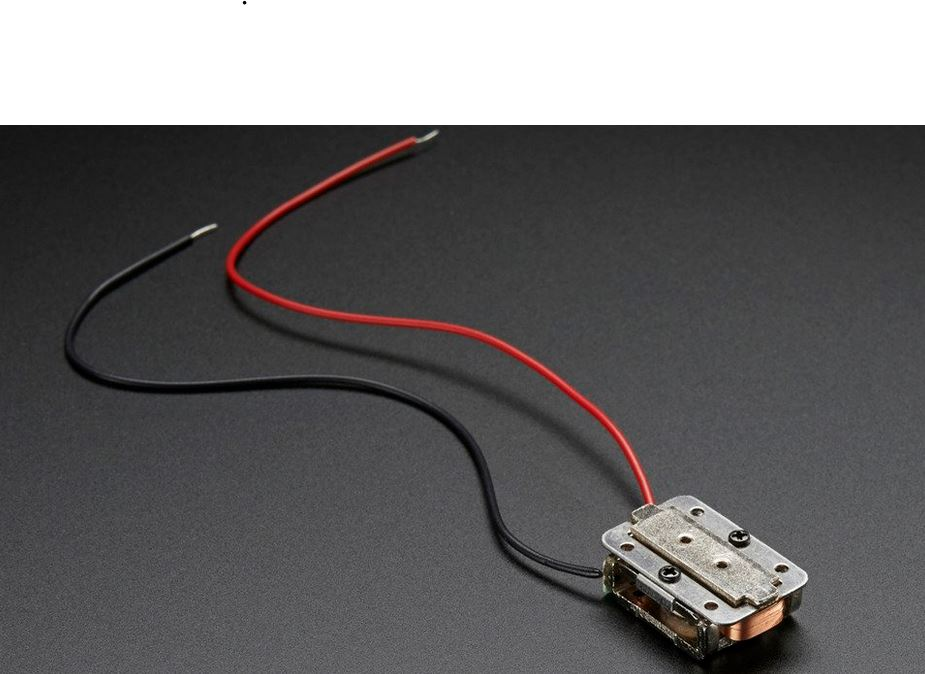
\includegraphics[width=6cm]{Bilder/Bone-Conductor.jpg}
	\caption[Bone Conductor]{Bone Conductor \cite{BoneConductor}}
	\label{Bone-Conductor}
\end{figure}

In der Abbildung \ref{Bone-Conductor} ist der für den Dojo benötigten Bone Conductor abgebildet. Der Bone Conductor ermöglicht es durch die Vibrationen, dass eine Audio Datei über den Schädelknochen abgespielt wird und so nur für eine Person hörbar ist, diese jedoch immer noch die Umgebungsgeräusche wahrnimmt. \cite{BoneConductor}



\section{Konzept}\label{AudioKonzept}
Das Konzept der Audioausgabe ist wie folgt aufgebaut:
\begin{figure}[h]
	\centering
	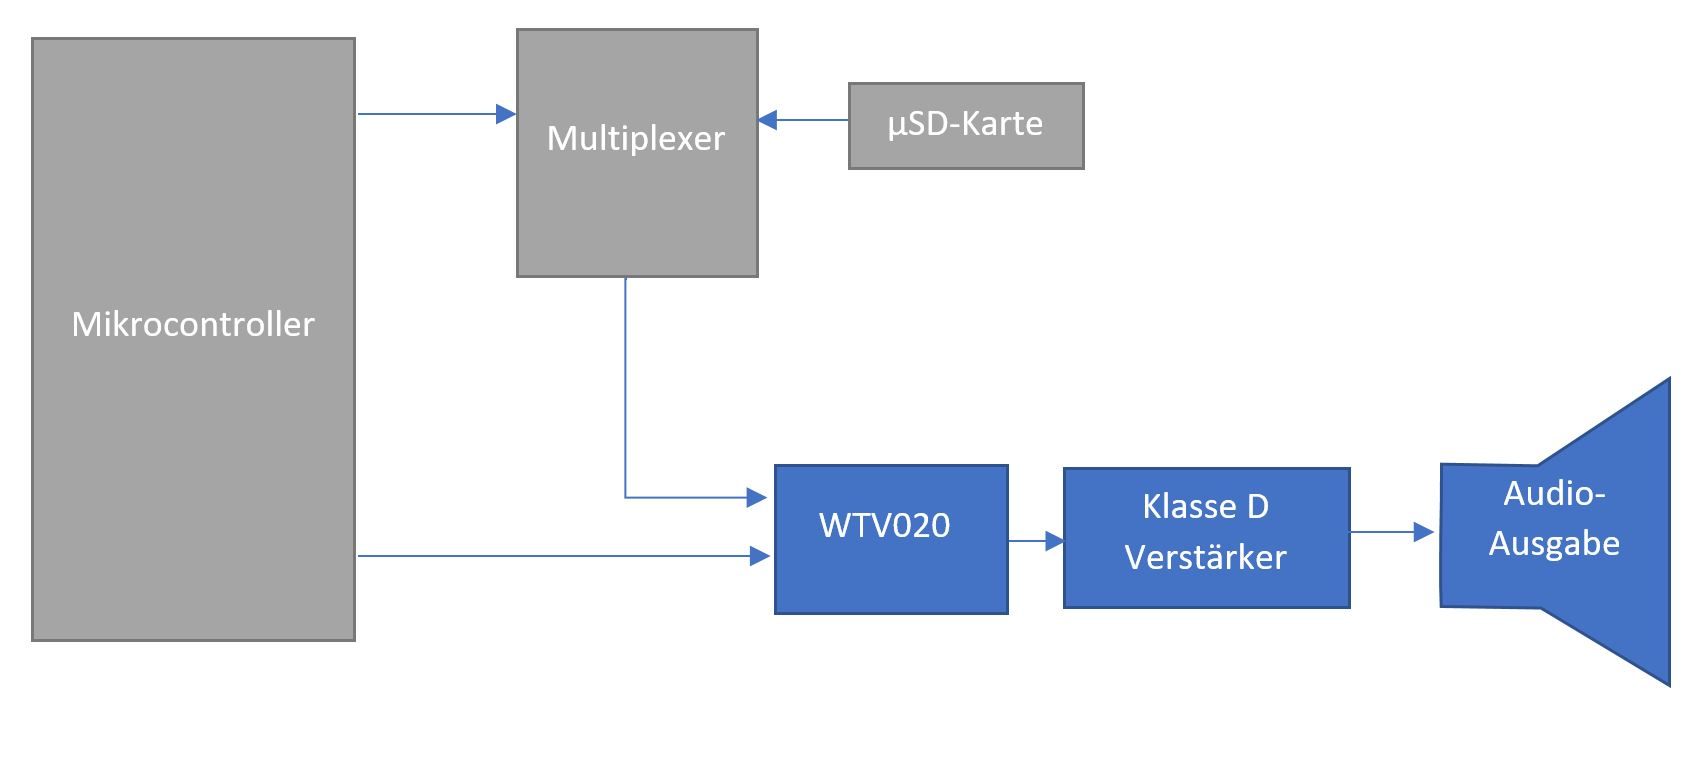
\includegraphics[width=11cm]{Bilder/Audio-Konzept.jpg}
	\caption{Audio Konzept}
	\label{Audio-Konzept}
\end{figure}\\
Die auf einer $\mu$SD-Karte abgespeicherten Audiodateien werden über einen Multiplexer, welcher vom Mikrocontroller gesteuert wird, an einen WTV020 Chip übertragen. Dieser wird in einem Serial Mode \ref{TechWTV} betrieben und kann ebenfalls vom Mikrocontroller angesteuert werden. Der Audiochip entschlüsselt die Daten und gibt diese an einen Klasse D Verstärker weiter. Dieser wird benötigt, um eine gut hörbare Lautstärke zu erreichen. Das Audiosignal wird schliesslich an einem Bone Conductor ausgegeben. 
Nachfolgend wird die Anordnung auf dem Print der einzelnen Komponenten dargelegt. 
\section{Hardware}
Wie im Konzept \ref{AudioKonzept}
 beschrieben, muss man, um Daten von der $\mu$SD-Karte auszulesen zuerst den Multiplexer ansteuern. Dies geschieht über den Mikrocontroller. Im ungesteuerten Zustand ist der MUX auf den WTV020-Chip geschaltet. Der WTV020SD-20S Chip kann nun auf die $\mu$SD-Karte zugreifen. Über vier Pins werden die Audiofiles ausgelesen und weitergegeben. Das Audiosignal wird auf den Klasse-D Verstärker gegeben. Dieser ist wie folgt aufgebaut.
\begin{figure}[h!]
	\centering
	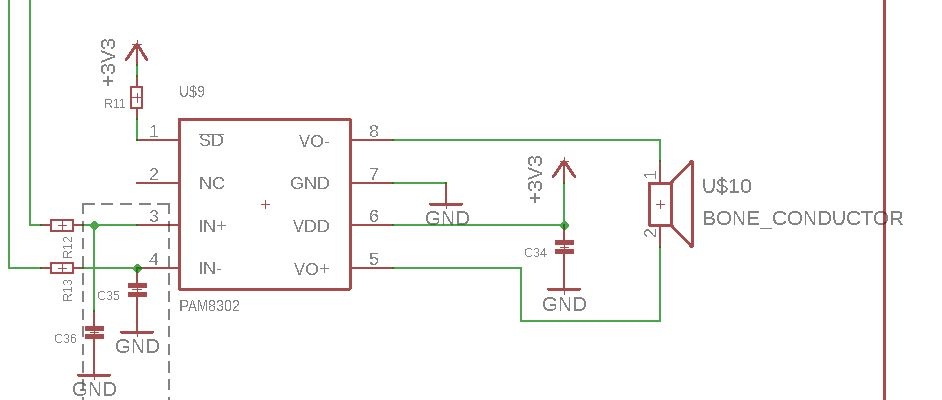
\includegraphics[width=10cm]{Bilder/Klasse-D.jpg}
	\caption{Klasse D Verstärker}
	\label{Klasse-D}
\end{figure}


Um ein Rauschen an der Speisung zu vermeiden, wird ein 1$\mu$ Farad grosser Kondensator benötigt. In diesem Projekt wurde zuerst eine konstante Verstärkung mit dem Faktor ca.10 verwendet, da die Lautstärken Regelung über den WTV020-Chip geregelt werden soll. Dieser Faktor entsteht aus dem Verhältnis des Internen Widerstandes und den zugeschalteten Widerständen. Um das Rauschen der Eingänge, sowie zu hohe Frequenzen zu filtern wurden zuerst wie die Abbildung \ref{Klasse-D} zeigt, Kapazitäten eingeplant. Auf dem Prototyp wurden aufgrund von Tests welche in der Validierung aufgeführt werden, die Vorwiderstände durch Kapazitäten ersetzt und die geplanten Kapazitäten weggelassen.\\ Wie erwähnt wird die Lautstärkenregelung über den WTV020-Chip geregelt. Dies ist jedoch im serial mode fehleranfällig. Übergangsweise wurde um die Lautstärke zu dämmen ein 50 Ohm grosser Widerstand vor den Bone Conductor geschaltet. Die Audioausgabe kann also wie beschrieben mit dem Bone Conductor umgesetzt werden.

\section{Firmware}
Wie im Kapitel Hardware beschrieben muss der MUX angesteuert werden um dem WTV-Chip den Zugriff auf die $\mu$SD-Karte zu gewähren. Im Kapitel \ref{USB} in der Tabelle \ref{truth_table_sd} ist beschrieben wie der MUX angesteuert werden muss, damit die benötigten Pins durchgeschaltet sind.
Für die Audioausgabe müssen alle Öffner geschlossen werden. Dies wird über die Pins 25 – 27 (Port C) realisiert. Sobald Musik abgespielt werden muss, werden die benötigten Ausgänge gesetzt. Das  WTV020 Modul vergleicht die Daten und Clock Pins wie folgt :
\begin{figure}[h]
	\centering
	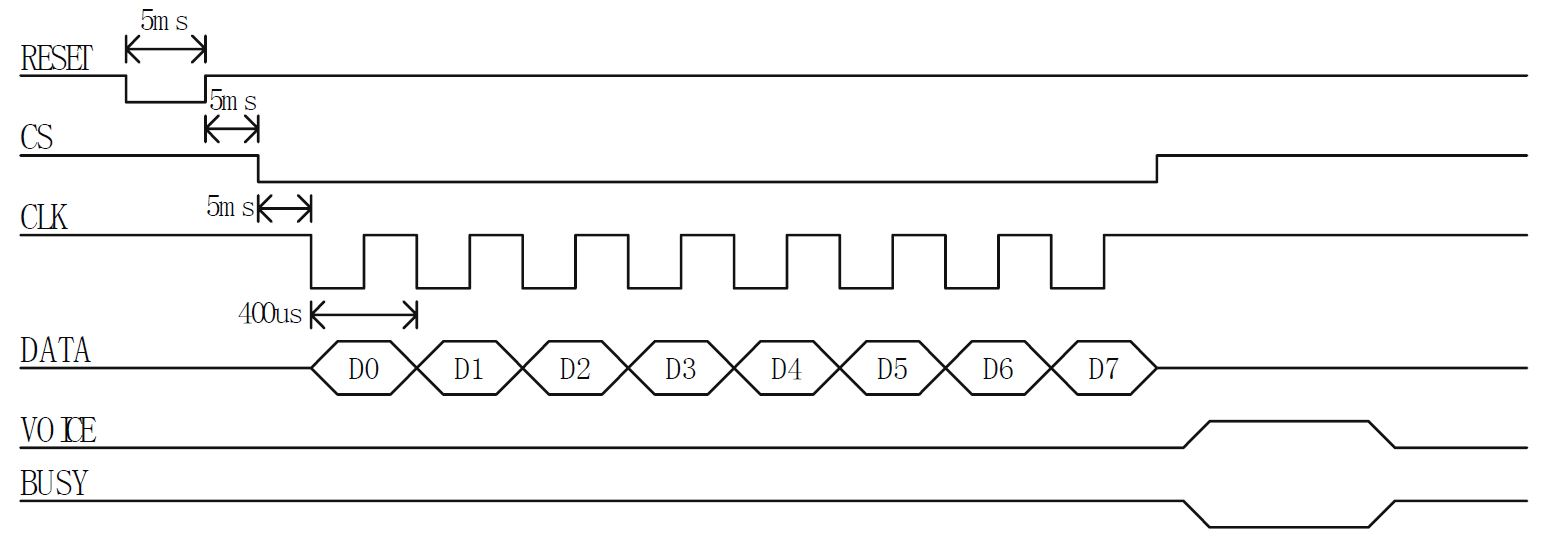
\includegraphics[width=15cm]{Bilder/WTV-Serial-Mode.JPG}
	\caption{WTV Serial Mode}
	\label{WTV-Serial}
\end{figure}\\
In der Abbildung \ref{WTV-Serial} ist ein three line serial mode dargestellt. Für den benötigten two line serial mode wird der CS Pin nicht benötigt.
\newpage
Sobald am Pin 7 über einen Taster Play ein low Signal erkannt wird, wird folgende Funktion aufgerufen:

\begin{figure}[h]
	\begin{verbatim}
void sendWTVcommand(unsigned int command){
	digitalWrite(WTV_CLK, LOW);
	_delay_us(1900);
	for (byte i = 0; i < 16; i++)
	{
		_delay_us(100);
		digitalWrite(WTV_CLK, LOW);
		digitalWrite(WTV_DOUT, LOW);
		if ((command & 0x8000) != 0)
		{
			digitalWrite(WTV_DOUT, HIGH);
		}
		_delay_us(100);
		digitalWrite(WTV_CLK, HIGH);
		command = command<<1;
	}
}
	\end{verbatim}
	\caption[Audio Datei abspielen]{Audio Datei abspielen \cite{WTVCODE}}
	\label{WTV-Play}
\end{figure}


Die benötigten Befehle welche sendWTVcommand mitgegeben werden müssen sind aufgrund des WTV020-Chips vorgefertigt.
Nachfolgend werden die verwendeten Befehle und deren Funktion aufgeführt.\\

	
\begin{table}[h]
	\centering
	\begin{tabular}{|c|c|} 
		Funktion & Befehl\\ 
		\hline 
		Play\_Pause & 0xFFFE \\ 
		\hline 
		STOP & 0xFFFF \\ 
		\hline 
		VOL & 0xFFF0-0xFFF7 \\ 
	\end{tabular} 
	\caption{WTV020 Funktionen}
	\label{WTVFunktionen}
\end{table} 

Bei der Funktion Play\_Pause ist zu erwähnen, dass um die Ausgabe zu starten am Anfang die gewünschte File Nummer gesendet werden muss (0-512). Ohne File Nummer wird die aktuelle Audioausgabe pausiert und kann wieder gestartet werden.

\section{Validierung}
Um die Audioausgabe zu testen, wurden verschiedene Versuche durchgeführt. Zuerst wurde der Bone Conductor über eine kleine Verstärkerschaltung direkt an einem Laptop angeschlossen, um die benötigte Leistung und die Lautstärke abschätzen zu können. Bei diesen Messungen ergab sich, bei einer sehr gut hörbaren Lautstärke, eine maximale Scheinleistung von 0.28 VA.\\
Um das WTV020 Modul mit geringem Aufwand zu testen wurde dieses zuerst im MP3 Mode betrieben.
So konnten schon am Anfang nicht kompatible $\mu$SD-Karten aussortiert werden. \\
Alle Funktionen des WTV020-Chips wurden separat und im two line serial mode überprüft. Alle verlangten Funktionen des Chips laufen Wunschgemäss. Zudem wurde ein Versuchsaufbau mit dem D-Klasse Verstärker durchgeführt, mit welchem die aktuell maximal benötigte Leistung von 1W gemessen wurde. \\
Trotz der funktionierenden Tests ist aktuell am Prototyp die Lautstärkenregelung nicht möglich. Das Audiomodul übernimmt die eingestellte Lautstärke, setzt diese jedoch, sobald das Gerät an einen Verstärker angeschlossen ist, vorherigen Wert zurück. Zudem ist zu erwähnen, dass für eine Massenproduktion ein WTV020 Modul nicht geeignet wäre, aufgrund der erwähnten Eigenheiten. Das Modul nimmt trotz gleicher Formatierung und gleichem Hersteller nicht jede $\mu$SD-Karten an. Zudem treten beim serial mode immer wieder kleiner Ungereimtheiten auf, wie z.B. die Lautstärkenregelung. 
